\documentclass[12pt]{report}
\usepackage{amsmath}
\usepackage{graphicx}
\begin{document}




%-----------------------------------------------------------------------
\chapter{The material optimzier }\label{sec:matopt}

\section{The mrun command}\label{sec:mrundesc}
The \verb+mrun+ command 

%-----------------------------------------------------------------------
\chapter{The material description}\label{sec:matdesc}



\section{The mparcart command}\label{sec:mparcartdesc}

The \verb+mparcart+ defines a material that is discretized on a coarse Cartesian grid, 
below refered to as the ``material grid''. The parameters are the offset values of 
$\rho$, $\mu$, and $\lambda$ relative a reference material, at the points of this grid. 
The material on the computational grid 
is defined by trilinear interpolation from the values on the coarser material grid. 
For example, the density, $\rho$, at a grid point $(i,j,k)$ in the computational grid is 
$$
  \rho_{i,j,k} = I(\{d^{(\rho)}\},x_i,y_j,z_k) + \rho^{(0)}_{i,j,k}
$$
where $\rho^{(0)}$ is the reference material, and $d^{(\rho)}$ is the difference $\rho-\rho^{(0)}$ 
on the material grid. The interpolation operator
$$
 I(\{ u \}, x,y,z)
$$
evaluates a function $u$ defined at the points of the material grid, at the point $(x,y,z)$.
\par
The number of points in the material grid, and initial values for $d^{(\rho)}, d^{(\mu)}, d^{(\lambda)}$
are specified by the \verb+mparcart+ command. For example
\begin{verbatim}
mparcart nx=5 ny=5 nz=3 init=0
\end{verbatim}
defines a material grid with $5\times 5\times 3$ points, and with $d^{(\rho)}$, $d^{(\mu)}$, $d^{(\lambda)}$
initialized to zero at all points.
The reference material is specified by one of the material commands 
of \emph{SW4}, e.g., \verb+block+ or \verb+pfile+, see the \emph{SW4} User's Guide for a
complete description of these material commands.

\par
Using a coarse material grid reduces the number of unknowns, compared with using the 
material at each grid point as parameters. Furthermore, the resolution in the material
is limited in terms of highest frequencies of the computed wave field, making it unreasonable
to expect to resolve the material down to the resolution of the computational grid.
We recommend that the grid spacing of the material grid is around 10 times 
the grid spacing of the computational grid. Also to note, the grid spacing of the material 
grid do not need to have any relation to the spacing of the computational grid. 
These two grids are independent.
\par
\begin{figure}
\begin{center}
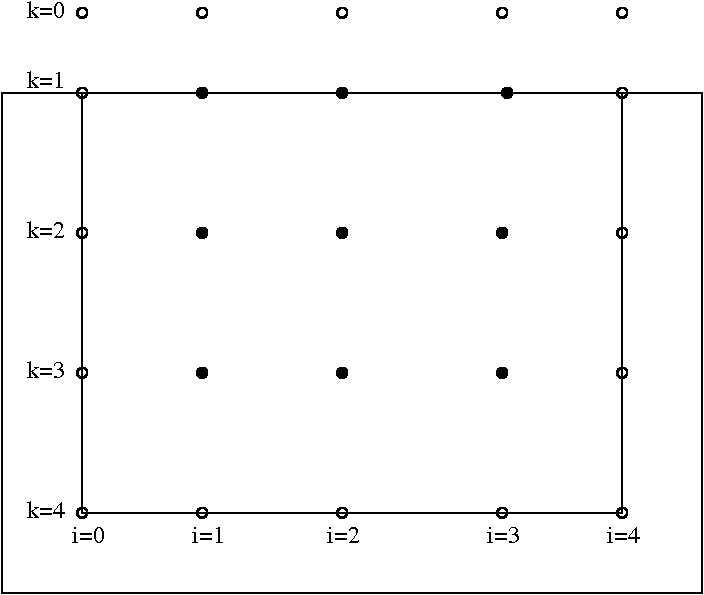
\includegraphics[width=0.8\textwidth]{mparcart.png}
\caption{Two dimensional slice of a material grid with $n_x=n_y=n_z=3$. The free surface boundary
is at $k=1$, there are super-grid sponge layers on the other sides. Filled circles indicate unknown
parameters, open circles are fixed boundary values.}
\label{fig:mparcart}
\end{center}
\end{figure}
\par
The material grid discretizes only the interior part the domain, without the super-grid
sponge layers. The configuration is outline in Fig~\ref{fig:mparcart} below.
The material grid is given by
\begin{alignat}{2}
 x_i = x_{min}+ i h_x \qquad i=0,\ldots,n_x+1\\
 y_j = y_{min}+ j h_y \qquad j=0,\ldots,n_y+1\\
 z_k = z_{min}+ k h_z \qquad k=0,\ldots,n_z+1
\end{alignat}
where the grid spacings $h_x$, $h_y$, and $h_z$ are determined such that $x_0, y_0, x_{n_x+1}, y_{n_y+1}$,
and $z_{n_z+1}$ are located at the interface between the interior domain and the super-grid sponge layer. 
In the depth direction, $z_1$ is on the free surface and, hence $z_{min}=-h_z$. The point $z_0$ is above the 
topography, but it will never be used in the interpolation. 

At the first and last points in each direction, ($i=0$, $j=0$, $k=0$, $n_x+1$, $n_y+1$, and $n_z+1$),
the offsets $d^{(\rho)}, d^{(\mu)}$, and $d^{(\lambda)}$ are fixed at zero, hence these values are
not part of the parameter vector. The total number of unknowns for the material inversion
is $3 \times n_x \times n_y \times n_z$.


%-----------------------------------------------------------------------
\chapter{Keywords in the input file}\label{chap:keywords}
The syntax of the input file is the same as in the forward solver, \emph{SW4}. The input
file consists of a number of lines with statements
\begin{verbatim}
command1 parameter1=value1 parameter2=value2 ... parameterN=valueN
# comments are disregarded
command2 parameter1=value1 parameter2=value2 ... parameterM=valueM
...
\end{verbatim}
Each command starts at the beginning of the line and ends at the end of the same line. Blank and
comment lines are disregarded. A comment is a line starting with a \# character. The order of the
parameters within each command makes no difference. 

Parameter values are either integers (-2,0,5,...), real numbers (20.5, -0.05, 3.4e4), or strings
(earthquake, my-favorite-simulation). Note that there must be no spaces around the = signs and
strings are given without quotation marks and must not contain spaces. 

A breif description of all commands is given in the following sections. The commands marked as
[required] must be present in all \emph{SW4mopt} input files, while those marked as [optional] are just
that. 

\section{Material optimizer}

\subsection{The mrun command}\label{sec:mrun}
\begin{flushleft}\bf
Syntax:\\
\tt
mrun task=... mcheck=... tsoutput=... 
\\
\bf Required parameters:\\
\rm
None
\end{flushleft}
The \verb+mrun+ command specifies which task to perform. The possible tasks are
given in the table below. 
\begin{center}
\begin{tabular}{|l|p{8cm}|l|l|l|} \hline
\multicolumn{2}{|c|}{\bf possible values of the task option}\\ \hline
{\bf Option} & {\bf Description}           \\ \hline 
\hline
minvert     & Perform material inversion (default) \\ \hline
gradtest    & Test gradient computation vs.~a numerical derivative \\ \hline
hesstest    & Compute the Hessian numerically  \\ \hline
func1d      & Compute and output a one dimensional cut of the misfit \\ \hline
func2d      & Compute and output a two dimensional surface of the misfit \\ \hline
forward     & Run one forward solve and exit. \\ \hline
\end{tabular}
\end{center}
Further specification of the {\tt func1d}, {\tt func2d} tasks, e.g., which parameter to
vary, can be done with the \verb+msurf+ command. The generated cut/surface is output on
a file named {\tt fsurf.bin}, the format of which is described in Section~\ref{}.
\par
The intended use of \verb+task=forward+ is to
generate synthetic seismograms for testing the material inversion. \par
\verb+mcheck=on+ tells the optimizer to check the computed material for reasonableness, e.g.,
that the density and $\mu$ are positive, after each iteration. \verb+tsoutput=on+ causes
the time series (synthetic seismograms) to be output after each iteration.
\verb+mcheck+ and \verb+tsoutput+ are only effective when the task is \verb+minvert+.
\begin{center}
\begin{tabular}{|l|p{6cm}|l|l|l|} \hline
\multicolumn{4}{|c|}{\bf mrun command parameters}\\ \hline
{\bf Option} & {\bf Description}          & {\bf Type} & {\bf Default} \\ \hline 
\hline
task    & task to perform                 & string & minvert \\ \hline
mcheck  & material checking (on or off)   & string & off \\ \hline
tsoutput & output time series (on or off) & string & off \\ \hline
\end{tabular}
\end{center}

Currently, mcheck only outputs diagnostic messages, no attempt to correct the material if
it is out of range is made.

\subsection{The lbfgs command}\label{sec:lbfgs}
\begin{flushleft}\bf
Syntax:\\
\tt
lbfgs nvectors=... ihess0=... maxit=... tolerance=... linesearch=...
\\
\bf Required parameters:\\
\rm
None
\end{flushleft}
Configure the L-BFGS method for minimizing the misfit. L-BFGS will iterate until \verb+maxit+ iterations
are reached, or until the maximum norm of the scaled gradient of the misfit is less than \verb+tolerance+. 
\par
The option {\tt linesearch=off} switches off the line search step of L-BFGS. This is usually not stable.
The default {\tt linesearch=on} switches on a standard line search algoritm. However, L-BFGS is only guaranteed to
be stable if the so called Wolfe condition is satisfied. The option {\tt linesearch=wolfe} switches on
the line search with additional logic to satisfy the Wolfe condition. Line search with the Wolfe condition 
is computationally expensive, since the gradient of the misfit has to be evaluated at least once. Therefore,
it is advisable to try the standard line search first, we have found it to work satisfactory in many cases.
\par
L-BFGS builds and approximation of the inverse Hessian, represented by \verb+nvectors+ vectors, which can
be thought of as a rank-\verb+nvectors+ approximation. The convergence rate is usually better for larger 
values of \verb+nvectors+. The method requires an initial guess for the inverse Hessian. The option
{\tt ihess0=scale-factors} uses an initial guess based on the scale factors of the problem, while
{\tt ihess0=gamma} uses an initial guess by an estimate of the size of the Hessian along the search 
directions, given by formula (7.20) in \cite{Nocedal-Wright}.

\begin{center}
\begin{tabular}{|l|p{7cm}|l|l|l|} \hline
\multicolumn{4}{|c|}{\bf lbfgs command parameters}\\ \hline
{\bf Option} & {\bf Description}          & {\bf Type} & {\bf Default} \\ \hline 
\hline
nvectors   & Number of l-bfgs vectors to keep & int   & 10 \\ \hline
ihess0     & Initial guess for inverse Hessian & string & gamma \\ \hline
maxit      & Maximum number of iterations  & int & 10 \\ \hline
tolerance  & Termination criterion for gradient  & float & $10^{-12}$ \\ \hline
linesearch  & Line search method (on, off, or wolfe)  & string & on \\ \hline
\end{tabular}
\end{center}

\subsection{The nlcg command}\label{sec:nlcg}
\begin{flushleft}\bf
Syntax:\\
\tt
nlcg maxit=... tolerance=... linesearch=... subtype=... maxsubit=...
\\
\bf Required parameters:\\
\rm
None
\end{flushleft}
Configure the non-linear conjugate gradient (NLCG) method for minimizing the misfit. NLCG will iterate 
until \verb+maxit+ restarts are reached, or until the maximum norm of the scaled gradient of the 
misfit is less than \verb+tolerance+. CG methods are usually restarted every $n$th iteration, 
where $n$ is the number of unknowns. The behavior of the iterations is controlled by the two 
parameters \verb+maxit+ and \verb+maxsubit+. \verb+maxit+ gives the maximum number of restarts, 
and \verb+maxsubit+ is the number of iterations between the restarts. By default \verb+maxsubit+ 
is set to $n$. 
\par
The option {\tt linesearch=off} switches off the line search step in NLCG. 
The default {\tt linesearch=on} switches on a standard line search algoritm. 
The initial step size is computed by approximating the minimization functional by
a quadratic surface.
\par
The \verb+subtype+ option makes it possible to specify the Fletcher-Reeves or the
Polak-Ribi\`ere variants of the NLCG. The Polak-Ribi\`ere algorithm forces a restart
more often than Fletcher-Reeves. With {\tt subtype=polak-ribiere}, \verb+maxit+ needs to 
be set large enough to allow for the additional restarts. 

\begin{center}
\begin{tabular}{|l|p{6cm}|l|l|l|} \hline
\multicolumn{4}{|c|}{\bf nlcg command parameters}\\ \hline
{\bf Option} & {\bf Description}          & {\bf Type} & {\bf Default} \\ \hline 
\hline
maxit       & Maximum number of iterations        & int & 10 \\ \hline
tolerance   & Termination criterion for gradient  & float & $10^{-12}$ \\ \hline
linesearch  & Line search method (on or off)  & string & on \\ \hline
subtype     & fletcher-reeves or polak-ribiere & string  & polak-ribiere \\ \hline
maxsubit    & Number of subiterations in CG & int & \# unknowns \\ \hline
\end{tabular}
\end{center}

\subsection{The mscalefactors command}\label{sec:nlcg}
\begin{flushleft}\bf
Syntax:\\
\tt
mscalefactors rho=... mu=... lambda=... file=... misfit=...
\\
\bf Required parameters:\\
\rm
None
\end{flushleft}
Introducing scale factors will improve the convergence rate of the minmizer, by reducing the condition number of 
the Hessian of the misfit. For quadratic problems, the scale factors form a diagonal pre-conditioning
matrix. There is one scale factor for each unknown. Ideally, the scale factor for the $i$th unknown, $x_i$, 
should be $1/\sqrt{H_{ii}}$, where $H_{ii}$ is the $i$th diagonal element of the Hessian. 
The \verb+file=+ option specifies a file name, from which the scale factors are read. The number of scale
factors on the file should be equal to the number unknown parameters. The format of the file is described
in Section~\ref{}.
\par
If the Hessian is not known, an alternative is to set the scale factors to reference sizes of the parameters.
If the material parameterization is made such that each parameter is identifiable with one of the material
properties, $\rho$, $\mu$, or $\lambda$, the options \verb+rho=+, \verb+mu=+, and \verb+lambda=+  can be
used to specify three different scales. These scale factors are used throughout for all unknowns of 
the respective type.
\par
The \verb+misfit=+ is a factor that modifies the input scale factors. It is based on the observation that
the scale of $1/\sqrt{H_{ii}}$, with $H=\partial^2f/(\partial x_i^2)$, is actually $x_r/\sqrt{f_r}$, where
$x_r$ is the scale of the unknown $x_i$, and $f_r$ is the scale of the objective function. All input
scale factors will be divided by the square root of the value of the \verb+misfit+ parameter.
The condition number of the Hessian is not affected by multiplying all factors by a constant, 
but the multiplier will affect the maximum step length, and is currently needed to sometimes reduce the 
allowed step size. This is a temporary measure that should be removed, once the line search algorithm
has been improved.

\begin{center}
\begin{tabular}{|l|p{6cm}|l|l|l|} \hline
\multicolumn{4}{|c|}{\bf mscalefactors command parameters}\\ \hline
{\bf Option} & {\bf Description}          & {\bf Type} & {\bf Default} \\ \hline 
\hline
rho      & Density scale factor                & float & 1 \\ \hline
mu       & Scale of Lam\'e parameter $\mu$     & float & 1 \\ \hline
lambda   & Scale of Lam\'e parameter $\lambda$ & float & 1  \\ \hline
file     & Name of file containing scale factors  & string  & None \\ \hline
misfit & Multiplier for scale factors & float & 1 \\ \hline
\end{tabular}
\end{center}

\subsection{The mfsurf command}\label{sec:nlcg}
\begin{flushleft}\bf
Syntax:\\
\tt
mfsurf var=... i=... j=... k=... pmin=... pmax=... npts=... var2=... i2=... j2=... k2=... pmin2=... pmax2=... npts2=...
\\
\bf Required parameters:\\
\rm
None
\end{flushleft}
The command \verb+mfsurf+ controls the selections for {\tt mrun task=func1d} and {\tt mrun task=func2d}.
The command assumes that the material parameters can be interpreted as values of
$\rho$, $\mu$, or $\lambda$ on a logically rectangular grid, for example, when using material
parameterization by the \verb+mparcart+ command.\par
\verb+var=+, \verb+i=+, \verb+j=+, \verb+k=+ specify one parameter. For example the density at the
point with index $(3,2,4)$ in the coarse material grid defined by \verb+mparcart+, is selected by
\begin{verbatim}
mfsurf var=rho i=3 j=2 k=4
\end{verbatim}
The command 
\begin{verbatim}
mfsurf var=rho i=3 j=2 k=4 npts=30 pmin=-250 pmax=250
\end{verbatim}
specifies the misfit as function of this parameter on the interval [-250,250], discretized by 30 points.
To compute and save the specified function on a file, run \emph{SW4mopt} with \verb+mrun task=func1d+.
\par
The second set of input variables, \verb+var2=+, \verb+i2=+, etc. are used for the second dimension when
a two dimensional misfit surface is specified with \verb+mrun task=func2d+.
\begin{center}
\begin{tabular}{|l|p{6cm}|l|l|l|} \hline
\multicolumn{4}{|c|}{\bf mfsurf command parameters}\\ \hline
{\bf Option} & {\bf Description}          & {\bf Type} & {\bf Default} \\ \hline 
\hline
var     & variable (rho, mu, or lambda)      & string & rho \\ \hline
i       & $i$-index                          & int & 1 \\ \hline
j       & $j$-index                          & int & 1 \\ \hline
k       & $k$-index                          & int & 1 \\ \hline
pmin    & lower parameter limit              & float & -300 \\ \hline
pmax    & upper parameter limit              & float &  300 \\ \hline
npts    & Number of discretization points    & int & 10  \\ \hline
var2    & variable (rho, mu, or lambda)      & string & rho \\ \hline
i2       & $i$-index                          & int & 1 \\ \hline
j2       & $j$-index                          & int & 1 \\ \hline
k2       & $k$-index                          & int & 2 \\ \hline
pmin2    & lower parameter limit              & float & -300 \\ \hline
pmax2    & upper parameter limit              & float &  300 \\ \hline
npts2    & Number of discretization points    & int & 10  \\ \hline
\end{tabular}
\end{center}


\section{Material parameterization [required]}
Several ways to parameterize the material will be tried. Currently, only parameterization through a
coarser grid is possible, by the \verb+mparcart+ command.

\subsection{mparcart}\label{sec:mparcart}
\begin{flushleft}\bf
Syntax:\\
\tt
mparcart nx=... ny=... nz=... init=...
\\
\bf Required parameters:\\
\tt
nx, ny, nz, init
\end{flushleft}
%
The command mparcart defines the material by interpolation from a coarse grid.
The coarse grid stores the offsets in $\rho$, $\mu$ and $\lambda$ from a reference material.
The init parameter is either 0, meaning that all offsets are initialized to zero, or the
name of a file with previously computed offsets. If a file name is specified, the material is
initialized with the values stored on the file. The material optimizer stores the current values
of the offsets on the file {\tt parameters.bin} after each iteration. Hence, a previous
computation can be restarted by specifying \verb+init=parameters.bin+.
\begin{center}
\begin{tabular}{|l|p{8cm}|l|l|l|} \hline
\multicolumn{4}{|c|}{\bf mparcart command parameters}\\ \hline
{\bf Option} & {\bf Description}          & {\bf Type} & {\bf Default} \\ \hline 
\hline
nx          & Number of points in $x$   & int    & none \\ \hline
ny          & Number of points in $y$   & int    & none \\ \hline
nz          & Number of points in $z$   & int    & none \\ \hline
init        & initial guess, file name or 0 & string & none \\ \hline
\end{tabular}
\end{center}

Currently, the complete material grid is stored in each processor. For very large problem sizes, the amount 
of memory can be a limitation. TODO: Implement a material grid, which is distributed on the processors.

\section{Output}

\subsection{mimage}\label{sec:mimage}
\begin{flushleft}\bf
\bf Syntax:\\ \tt mimage x=... y=... z=... cycle=... cycleInterval=... file=... mode=... precision=...\\
 \bf Required parameters:\\ 
\rm Location of the image plane (x, y, or z) \\ 
Time for output (cycle, or cycleInterval)\\ 
\end{flushleft}
%
Material images are similar to the image command of \emph{SW4}. The main difference is that \verb+mimage+ 
defines image output related to the iterations of the minimization algorithm. In the {\tt cycle} 
and {\tt cycleInterval} options, one cycle is interpreted as one iteration of the minimization algorithm.
The options {\tt x}, {\tt y}, {\tt z}, {\tt file}, {\tt mode}, and {\tt precision} are identical to
the options with the same names in the \verb+image+ command.
\verb+mimage+ only outputs images of material properties. The supported modes are given in the table below.
\begin{center}
\begin{tabular}{|c|l|} \hline
\multicolumn{2}{|c|}{\bf mimage mode options}\\ \hline
\bf{Value} & \bf{Description} \\ 
\hline  \hline
rho     & Density \\ \hline
lambda  & 1st Lam\'e parameter \\ \hline
mu      & 2nd Lam\'e parameter (shear modulus) \\ \hline
p       & Compressional wave speed \\ \hline
s       & Shear wave speed \\ \hline
gradrho     & Gradient of misfit w.r.t.\ density \\ \hline
gradlambda  & Gradient of misfit w.r.t.\ 1st Lam\'e parameter \\ \hline
gradmu      & Gradient of misfit w.r.t.\ 2nd Lam\'e parameter \\ \hline
gradp       & Gradient of misfit w.r.t.\ Compressional wave speed \\ \hline
grads       & Gradient of misfit w.r.t.\ Shear wave speed \\ \hline
%qp      & $Q_P$ quality factor \\ \hline
%qs      & $Q_S$ quality factor \\ \hline
\end{tabular}
\end{center}
Note, the misfit gradients are computed with respect to the material properties at each grid point.
When using a material parameterization, the misfit with respect to the parameters is given by the chain
rule as a combination of these gradients with the derivative of the parameterization. \par
\begin{center}
\begin{tabular}{|l|p{8cm}|l|l|l|} \hline
\multicolumn{4}{|c|}{\bf mimage command parameters}\\ \hline
{\bf Option} & {\bf Description}          & {\bf Type} & {\bf Default} \\ \hline 
\hline
cycle         & Minimizer cycle to output image $(\geq 0)$                     & int    & 0 \\ \hline
cycleInterval & Minimizer cycle interval to output a series of images $(\geq 1)$ & int   & 1 \\ \hline
file          & File name header of image                                   & string & mimage \\ \hline
precision     & Floating point precision for saving data (float or double)  & string & float \\ \hline
mode          & The field to be saved                                       & string & rho \\ \hline
\end{tabular}
\end{center}


 

\end{document}